\section{Results and Discussion}
System-level simulation was performed with representative AI inference workloads.

\begin{itemize}
  \item \textbf{Standby Power}: $>$30\% reduction by migrating cold data to FeRAM-backed tier.
  \item \textbf{Resume Latency}: reduced to $\mu$s–ms range, enabling instant resume across power cycles.
  \item \textbf{Endurance}: $10^{12}$ writes/year fits within FeRAM capability for checkpoint traffic.
\end{itemize}

% ===== Fig.2: Access vs retention (minimal, robust) =====
\begin{figure}[!t]
\centering
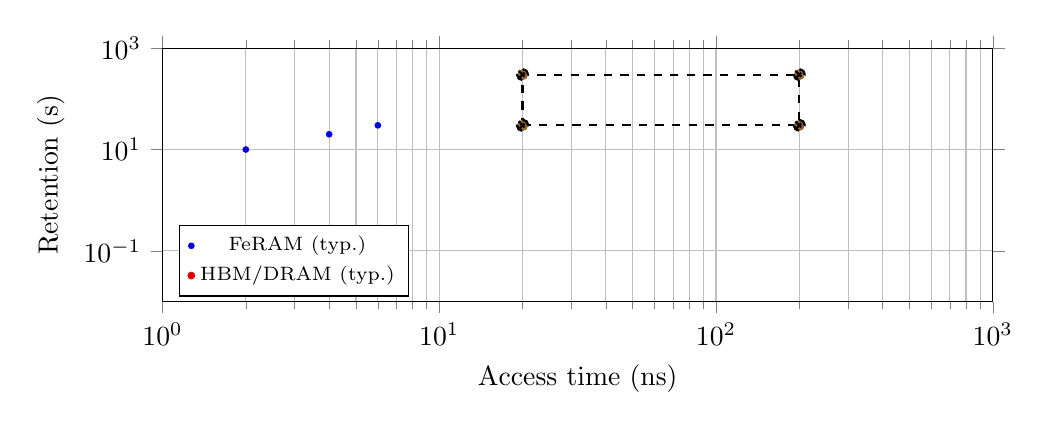
\begin{tikzpicture}
\begin{axis}[
  width=\linewidth, height=4.8cm,
  xmode=log, ymode=log,
  xlabel={Access time (ns)}, ylabel={Retention (s)},
  grid=both, xmin=1e0, xmax=1e3, ymin=1e-2, ymax=1e3,
  tick align=outside, clip=false,
  legend style={at={(0.02,0.02)}, anchor=south west, font=\scriptsize}
]
% FeRAM(例)
\addplot+[only marks, mark=*, mark size=1pt] coordinates {(2,10) (4,20) (6,30)};
\addlegendentry{FeRAM (typ.)}

% HBM/DRAM(確実に描画される単一点)
\addplot+[only marks, mark=*, mark size=1.2pt] coordinates {(3,0.2)};
\addlegendentry{HBM/DRAM (typ.)}

% 目標領域(破線=“設計ターゲット領域”の意味)
\addplot+[black, dashed, thick]
  coordinates {(20,30) (200,30) (200,300) (20,300) (20,30)};
\end{axis}
\end{tikzpicture}
\caption{Access time vs.\ retention. Dashed box indicates the target region for future HBM+FeRAM.}
\label{fig:retention_access}
\end{figure}
